\section{Camera Pose Calibration}\label{app:camera_pose_calibration}

For evaluation of sim-to-real transfer, the camera pose is calibrated with respect to the robot base frame. For this, a calibration board with ArUcO markers \cite{garrido-jurado_automatic_2014} is used as an intermediate reference. \autoref{app_fig:calibration_setup} shows the utilised setup. Position of this intermediate reference is first found in the robot coordinate system by positioning robot's tool centre point above origin of the calibration board, and using robot's joint encoders together with forward kinematics. Hereafter, ArUcO pattern is detected from RGB images of the utilised camera. The perceived pixel positions of the pattern are then used with its known design to solve a perspective-n-point problem and determine camera pose with respect to the pattern. Once known, pose of the camera is determined with respect to the robot and the calibration board is removed from the scene.

\setcounter{figure}{0}
\begin{figure}[ht]
    \centering
    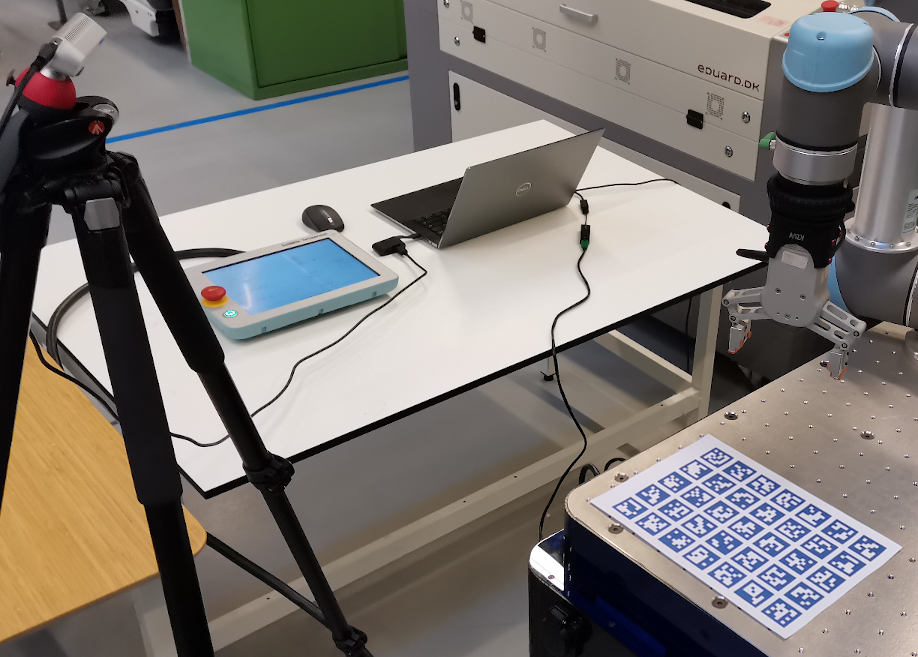
\includegraphics[width=1.0\textwidth]{experimental_evaluation/real_calibration_setup_cropped.png}
    \caption{Setup used for calibration, where ArUco markers are used as an intermediate reference frame between the camera and robot.}
    \label{app_fig:calibration_setup}
\end{figure}
